%% =====================================================================
%%  International Journal of Production Research (IJPR)
%%  Taylor & Francis "Interact" layout, APA reference style.
%%
%%  Compile with the official "Taylor & Francis Interact (APA)" bundle:
%%  keep interact.cls in the working folder (it ships with the template),
%%  together with this file and IJPR_CSLAP.bib. On Overleaf, start from the
%%  "Taylor & Francis Interact (APA reference style)" template and replace
%%  its main.tex and .bib with these two files.
%%
%%  References use BibTeX via apacite (natbibapa), exactly as documented in
%%  the template's main.tex; bibliographystyle = apacite (set below). Do NOT
%%  also load natbib: apacite's natbibapa option provides \citep / \citet.
%%
%%  Author note: replace the corresponding-author email and the Savoye
%%  city with the final submission details before upload.
%% =====================================================================
\documentclass[]{interact}

% interact.cls already loads amsmath, amssymb, amsfonts, amsthm, booktabs,
% epsfig, graphicx and rotating. We add only what this manuscript needs.
\usepackage{mathtools}
\usepackage{multirow}
\usepackage{algorithm}
\usepackage{algpseudocode}
\usepackage{tikz}
\usetikzlibrary{shapes.geometric, arrows.meta, positioning, calc}

% APA references via BibTeX, exactly as the interact-APA sample documents.
\usepackage[natbibapa,nodoi]{apacite}
\setlength\bibhang{12pt}
\renewcommand\bibliographytypesize{\fontsize{10}{12}\selectfont}

\begin{document}

\articletype{RESEARCH ARTICLE}

\title{Efficient and practical solutions for the correlated storage location assignment problem in automated pick-and-pass warehouses}

\author{
\name{Ermal Belul\textsuperscript{a,b}\thanks{CONTACT Ermal Belul. Email: ermalbeluli10@gmail.com}, Marwane Bouznif\textsuperscript{b}, Dritan Nace\textsuperscript{a} and Antoine Jouglet\textsuperscript{a}}
\affil{\textsuperscript{a}Universit\'{e} de technologie de Compi\`{e}gne, CNRS, Heudiasyc UMR 7253, Compi\`{e}gne, France; \textsuperscript{b}Savoye, France}
}

\maketitle

% ---------------------------------------------------------------------
% Unstructured abstract (<= 200 words, single paragraph)
% ---------------------------------------------------------------------
\begin{abstract}
Automated, conveyor-driven pick-and-pass warehouses are limited by mechanical station stops rather than by picker travel distance. We study the correlated storage location assignment problem (CSLAP) for these systems and replace the usual distance objective with the minimisation of station visits per order, subject to hard per-station capacity and workload limits. The problem is formulated as a mixed-integer linear programme and solved both with a branch-and-bound solver and with a set-variable reformulation handled by a hybrid local-search engine. A parameter-light clustering heuristic and a column-generation framework complete the method set, and every approach is benchmarked against a genetic algorithm and simulated annealing with correlated interchange over many random instances using paired statistical tests. On synthetic instances of 50 to 2000 stock-keeping units the set-variable approach is the best feasible method at every scale, and its advantage over the metaheuristics grows with problem size. On a real warehouse of 21,877 stock-keeping units and 26 stations it lowers station visits by 13.7 per cent while holding every station within capacity. A bounded reassignment extension then maps the trade-off between re-slotting effort and throughput, which supports non-disruptive continuous improvement on an active site.
\end{abstract}

\begin{keywords}
storage location assignment; pick-and-pass warehouse; warehouse automation; mixed-integer programming; column generation; metaheuristics
\end{keywords}

% =====================================================================
\section{Introduction}
% =====================================================================
Order picking absorbs a large share of warehouse operating cost, so where products sit on the shelves has a direct effect on throughput \citep{xie2024combi}. The correlated storage location assignment problem (CSLAP) chooses that placement by grouping products that are frequently ordered together, with the aim of shortening order preparation. Most CSLAP models pursue this aim by minimising the travel distance of the picker \citep{islam2023}. That objective is the right one when a human walks the aisles. It is the wrong one once the goods move on a conveyor.

In an automated pick-and-pass facility the movement of totes between zones is mechanised. The operational limit is no longer how far anyone walks but how often a tote is diverted, stopped, and merged back into the main line. Each diversion adds a fixed mechanical and handling delay and consumes a slot in a finite station buffer. The cost driver shifts from distance to the number of station visits per order, together with the balance of workload across zones. We take this shift as the starting point and build a CSLAP model whose objective is the total number of station visits, constrained so that no station exceeds its physical capacity or its daily workload budget.

Solving that model at the scale of a real catalogue is the difficulty. The objective counts discrete stops, so its value changes only when a whole order gains or loses a zone. The resulting landscape is flat and piecewise constant, which removes the gradient information that branch-and-bound and local search normally exploit. On instances beyond a few hundred products a standard binary formulation solved by branch-and-bound fails to improve on a feasible starting layout within practical time. The contribution of this paper is the methodology that gets past that wall, together with the evidence that it transfers to an operating site.

We make four contributions. First, we pose CSLAP for pick-and-pass systems with station visits as the objective and hard capacity and workload limits, and we give a mixed-integer linear programme for it. Second, we show that pairing a set-variable reformulation of that programme with a hybrid local-search engine scales to instances on which binary branch-and-bound stalls; at that scale branch-and-bound returns only a trivial lower bound, so we report solution quality relative to the best solution found across all methods rather than to a certified optimum. Third, we benchmark the set-variable approach against a clustering heuristic, a column-generation framework, a genetic algorithm (GA), and simulated annealing with correlated interchange (SA-C), over multiple random instances with paired statistical tests, and we validate it on a real warehouse of 21,877 products and 26 stations. Fourth, we add a bounded reassignment extension that limits how many products may move, which lets the gains be deployed gradually on an active facility.

The rest of the paper follows the structure expected of a production-research study. Section~\ref{sec:litreview} reviews the relevant production and logistics literature. Section~\ref{sec:model} defines the problem and the decision-aid model. Section~\ref{sec:methods} describes the solution methods. Section~\ref{sec:experiments} reports the synthetic benchmarking and the statistical tests. Section~\ref{sec:industrial} reports the industrial application. Section~\ref{sec:managerial} translates the results into managerial insight, and Section~\ref{sec:perspectives} sets out research perspectives.

% =====================================================================
\section{Related production research}\label{sec:litreview}
% =====================================================================
The move from manual picker-to-parts warehouses to automated, conveyor-driven, zone-picking systems changes which model is appropriate. In manual systems travel distance dominates, and CSLAP has accordingly been studied through distance minimisation \citep{islam2023, wang2020}. \citet{zhang2019cie} model demand correlation explicitly and place co-ordered products near a depot, and \citet{xiao2010correlated} use bill-of-material structure to the same end. These models remain the reference point for picker-to-parts settings.

Applying the same objective to automated architectures misreads the cost structure. In robotic mobile fulfilment systems and conveyor systems the goods are transported mechanically, so the system-level limits are the number of station visits, order splits, mechanical dwell, and the synchronisation of workload across zones \citep{azadeh2019, xie2021}. These bottlenecks originate in the per-diversion mechanical setup and in the queueing behaviour of the finite station buffers, both of which fall when an order visits fewer zones \citep{zhu2021, kim2020}. Section~\ref{sec:model} develops this conveyor model; here we review the prior models that target the same system-level metrics.

Recent work supports reframing the objective around discrete touches. \citet{zhu2021} minimise order splits across multiple warehouses by clustering, which maps directly to grouping products into conveyor zones so that an order stays intact. \citet{xie2021} present a mixed-integer programme that minimises pod-station visits and prove that fewer visits, combined with dispersed workload, raise system throughput. \citet{mirzaei2021} propose correlated dispersed storage, which spreads correlated items across automated assets to avoid a queue forming at any single workstation. The common thread is that reducing visits must be paired with workload balance, otherwise the optimisation overloads one zone.

Workload balance is therefore a constraint, not an afterthought. \citet{tarczynski2023} give linear-programming models that balance workload across pick-and-pass zones and show that balance is a precondition for reducing total picking time. \citet{pan2015} use a group genetic algorithm to balance zone workload during order batching, and \citet{vanGils2018} show by analysis of variance that storage assignment and zoning have to be optimised together. \citet{boysen2023} survey synchronisation in parts-to-picker systems and conclude that delivering each tote to a capacity-feasible station without queueing is the main determinant of throughput.

Because storage assignment with hard synchronisation is NP-hard, decomposition methods have gained ground. \citet{muter2022} formulate order batching and picker scheduling as a set-partitioning model solved by column generation, with workload pacing enforced inside the pricing problem, and \citet{zhen2025} design column-and-row generation for hard synchronisation constraints in autonomous-robot warehouses. These results show that station capacity and workload can be carried as resource limits inside a pricing subproblem, which is the route we follow for our own column-generation framework.

Table~\ref{tab:litreview} positions this paper against representative studies along the dimensions that matter for the automated setting: the objective, whether a hard per-station workload cap is enforced, the operational environment, the largest reported instance, and the solution method. The gap it identifies is not the visit objective, which several authors already advocate, but a method that solves the objective for a real catalogue of tens of thousands of products under hard workload limits, validated on an operating facility.

\begin{table}[t]
\centering
\tbl{Positioning of this study against representative storage-assignment and order-picking research.}
{\begin{tabular}{@{}lllll@{}}
\toprule
Study & Objective & Hard WL cap & Setting & Largest instance \\
\midrule
\citet{zhang2019cie}   & Travel distance       & No   & Manual, correlated      & Hundreds of SKUs \\
\citet{wang2020}       & Travel distance       & No   & Manual picker-to-parts  & Hundreds of SKUs \\
\citet{mirzaei2021}    & Dispersion/affinity   & Partial & Robotic fulfilment   & $\sim$10$^3$ SKUs \\
\citet{xie2021}        & Pod-station visits    & No   & Robotic fulfilment      & $\sim$10$^3$ items \\
\citet{tarczynski2023} & Picking time          & Yes  & Pick-and-pass           & Small to medium \\
\citet{muter2022}      & Makespan              & Yes  & Batching/picking        & Medium \\
This study             & Station visits        & Yes  & Pick-and-pass, automated & 21,877 real SKUs \\
\bottomrule
\end{tabular}}
\label{tab:litreview}
\end{table}

% =====================================================================
\section{Problem definition and decision-aid model}\label{sec:model}
% =====================================================================
We describe the operating system, define the decision in operational terms, and then state the mathematical programme. The notation is collected in Table~\ref{tab:notation}.

\subsection{The pick-and-pass picking section}
Orders travel along a main conveyor and pass a sequence of picking stations, each on a spur off the main line (Figure~\ref{fig:schematic}). A station holds a fixed set of products on nearby shelving. When an order needs a product stored at a station, its tote diverts onto the spur, an operator picks the required items into the tote, and the tote merges back into the main line. The tote repeats this at every station that holds one of its products, then leaves the section for dispatch. One such diversion is a \emph{station visit}, also called a station stop. An \emph{order split} happens when an order's products sit across more than one station, which forces more than one visit.

\begin{figure}[t]
\centering
\begin{tikzpicture}[
  font=\small,
  station/.style={draw, rounded corners, fill=black!6, minimum width=1.9cm, minimum height=0.95cm, align=center},
  bin/.style={draw, fill=black!15, minimum size=0.30cm, inner sep=0pt},
  conv/.style={line width=2pt, -{Latex[length=3mm]}, black!70},
  spur/.style={thick, -{Latex[length=2mm]}, black!55},
]
\draw[line width=6pt, black!12] (-0.2,0) -- (12.2,0);
\draw[conv] (-0.2,0) -- (12.6,0);
\node[left] at (-0.3,0) {Input};
\node[right] at (12.7,0) {Dispatch};
\node[below, font=\footnotesize] at (6.2,-0.28) {Main conveyor (orders advance in sequence)};
\node[station] (s1) at (2.4,2.25) {Station $s_1$};
\node[station] (s2) at (6.2,2.25) {Station $s_2$};
\node[station] (s3) at (10.0,2.25) {Station $s_{|S|}$};
\node[font=\scriptsize] at (8.2,2.25) {$\cdots$};
\foreach \x in {2.4,6.2,10.0}{
  \draw[spur] (\x-0.65,0.05) -- (\x-0.65,1.75);
  \draw[spur] (\x+0.65,1.75) -- (\x+0.65,0.05);
}
\node[font=\scriptsize, black!55, align=center] at (2.4,1.0) {divert $\uparrow$\\ merge $\downarrow$};
\foreach \x in {0.5,1.4,4.3,8.0,11.4}{ \node[bin] at (\x,0) {}; }
\node[font=\scriptsize] at (0.5,-0.55) {order tote ($P_o$)};
\node[bin] at (5.55,0.5) {};
\node[bin] at (5.55,0.86) {};
\node[align=center, font=\scriptsize] at (6.2,0.95) {finite\\ buffer};
\draw[step=0.27cm, black!45, thin] (1.45,2.95) grid (3.35,3.4);
\node[font=\scriptsize] at (2.4,3.62) {shelving: products stored at $s$};
\end{tikzpicture}
\caption{Schematic of a pick-and-pass picking section. A tote diverts onto a station's spur whenever that station stores one of the order's products $P_o$, is processed, then merges back; each diversion is one station visit. Concentrating co-ordered products at a shared station reduces both the number of visits and the occupancy of the finite station buffer.}
\label{fig:schematic}
\end{figure}

Two operational facts drive the model. A visit carries a fixed cost that is independent of how many items are picked, because the tote still has to be decelerated, inducted, scanned, and merged. Grouping co-ordered products at one station therefore collects more items per stop and lowers the visit count. At the same time, a station buffer has finite capacity, so concentrating too much traffic on one station lets its queue overflow and block the main line. Reducing visits is only safe if the workload on each station stays within a budget. Both effects are captured below: visits in the objective, workload in a hard constraint.

\subsection{Sets, parameters, and decisions}
Let $P$ be the catalogue of products, where each product is one stock-keeping unit (SKU); $O$ the set of orders observed over the planning horizon; and $S$ the set of stations, that is the picking zones. An order $o$ usually requests several products, collected in its line set $P_o \subseteq P$. The same product appears in many orders, and the demand of product $p$, written $L_p$, is the number of order lines in which it occurs over the horizon, in lines per day. Each station $s$ has a number of storage locations $\zeta_s$, a processing speed $V_s$ in lines per day, and a daily time budget $T_s$ expressed as a fraction of a working day. We model the placement at the station level: a product is assigned to exactly one station, and we do not fix which physical slot it occupies, since station shelving can be rearranged without changing the station's total capacity $\zeta_s$. A single station per product keeps inventory and replenishment simple; allowing high-demand products at several stations is left to Section~\ref{sec:perspectives}.

\begin{table}[t]
\centering
\tbl{Notation.}
{\begin{tabular}{@{}cl@{}}
\toprule
Symbol & Definition \\
\midrule
$P,\,O,\,S$ & Sets of products (SKUs), orders, and stations (zones) \\
$P_o$       & Set of products requested in order $o \in O$ \\
$\zeta_s$   & Number of storage locations at station $s$ \\
$L_p$       & Daily order lines for product $p$ (lines per day) \\
$V_s$       & Processing speed of station $s$ (lines per day) \\
$T_s$       & Daily time budget of station $s$ (fraction of a day) \\
$K_s$       & Set of feasible assignment patterns for station $s$ \\
$x_{ps}$    & 1 if product $p$ is assigned to station $s$ \\
$z_{os}$    & 1 if order $o$ visits station $s$ \\
\bottomrule
\end{tabular}}
\label{tab:notation}
\end{table}

\subsection{Mixed-integer linear programme}
The binary variable $x_{ps}$ is 1 when product $p$ is assigned to station $s$. The variable $z_{os}$ records whether order $o$ visits station $s$, and it is forced to 1 whenever any product of $o$ sits at $s$. The model is
\begin{align}
\min \quad & \sum_{o \in O} \sum_{s \in S} z_{os} \label{eq:obj}\\
\text{s.t.} \quad
& \sum_{s \in S} x_{ps} = 1 && \forall p \in P \label{eq:assign}\\
& \sum_{p \in P} x_{ps} \le \zeta_s && \forall s \in S \label{eq:cap}\\
& x_{ps} \le z_{os} && \forall o \in O,\ p \in P_o,\ s \in S \label{eq:link}\\
& \sum_{p \in P} x_{ps}\,\frac{L_p}{V_s} \le T_s && \forall s \in S \label{eq:wl}\\
& x_{ps} \in \{0,1\},\quad z_{os} \in [0,1]. && \label{eq:dom}
\end{align}
The objective \eqref{eq:obj} counts station visits across all orders. Constraint \eqref{eq:assign} assigns each product to one station, and \eqref{eq:cap} respects the physical capacity of each station. Constraint \eqref{eq:link} links visits to assignments: if a product of order $o$ is stored at $s$, then $o$ visits $s$. The objective drives $z_{os}$ to its lower bound, so it takes value 1 only when a visit is unavoidable, and it stays integral without a big-$M$ term even though it is declared continuous. Constraint \eqref{eq:wl} caps the daily workload of each station, where $L_p/V_s$ is the time product $p$ adds to station $s$. The workload sum runs over all products assigned to the station, not over a single order.

\subsection{Set-variable reformulation}\label{sec:setvar}
The same model can be expressed with set decision variables rather than a binary matrix \citep{blaisemodeling}. We introduce one set variable $\Phi_s$ per station whose value is the subset of products assigned to that station, so the matrix $x_{ps}$ is replaced by the family $\{\Phi_s\}_{s \in S}$. This reduces the number of declared variables from $|P|\times|S|$ to $|S|$. The reduction is in the representation, not in the combinatorial difficulty: the model still decides which of the $|P|$ products goes to which of the $|S|$ stations, and the problem stays NP-hard. The value is operational. A set representation exposes high-level operators (partition, contains, count) and a compact move space, which lets a hybrid local-search engine traverse the flat, piecewise-constant landscape more effectively than by flipping $|P|\times|S|$ individual binary flags. We solve this reformulation with the Hexaly engine and refer to it as the set-variable approach.

% =====================================================================
\section{Solution methods}\label{sec:methods}
% =====================================================================
Three methods solve the model: the set-variable reformulation of Section~\ref{sec:setvar}, a clustering heuristic, and a column-generation framework. They are benchmarked against the GA and SA-C baselines of Section~\ref{sec:baselines}.

\subsection{Greedy clustering heuristic}\label{sec:heuristic}
For very large catalogues we use a fast heuristic that builds tightly correlated communities of products and assigns them to stations. It extends the agglomerative idea of \citet{chuang2016}, which merges correlated items into clusters, but it builds disjoint communities by greedy graph connectivity \citep{west2001introduction} and adapts its thresholds to the size of the catalogue, so that a co-occurrence count that signals affinity in a 50-product instance is not mistaken for noise in a 20,000-product one.

Let $N = |P|$. The heuristic needs no per-instance tuning. It fixes a small set of constants and derives the operative thresholds from $N$: a preprocessing frequency floor $\max(2, \lfloor N/100 \rfloor)$, a minimum pairwise co-occurrence $\max(2, \lfloor N/50 \rfloor)$, a kept-edge ratio of $0.1$, and a community size bound $\max(5, \min(15, \lfloor N/20 \rfloor))$. Each constant tracks a fixed fraction of catalogue volume. Feasibility is governed by the station capacity $\zeta_s$ rather than by these correlation thresholds, to which the output is robust under moderate variation. The procedure has four stages: filter low-frequency noise and rank correlated pairs; grow disjoint communities from the strongest pair up to the size bound; sweep residual products into their most correlated community with room; then rank communities by demand and place them on stations by historical preference, splitting a community only when no single station can hold it. The full procedure is given in the appendix. The heuristic is fast and scalable, but it optimises affinity without the workload constraint \eqref{eq:wl}, so its raw output can breach the workload cap, as the experiments confirm.

\subsection{Column generation}\label{sec:cg}
For bounded solutions we adapt a set-covering column-generation framework \citep{lubbecke2005selected, desrochers1989column}. Columns are feasible product-station patterns, generated per station so that cross-station uniqueness is handled by the master rather than by every pricing call. Let $\delta_{psk}$ be 1 if product $p$ is in pattern $k$ of station $s$, and let $z_{osk}$ be 1 if any product of order $o$ is in that pattern. With $y_{sk}=1$ when pattern $k$ is selected for station $s$, the restricted master problem is
\begin{align}
\min \quad & \sum_{o \in O}\sum_{s \in S}\sum_{k \in K_s} z_{osk}\,y_{sk}\\
\text{s.t.}\quad
& \sum_{k \in K_s} y_{sk} \le 1 && \forall s \in S \quad (\pi_s)\\
& \sum_{s \in S}\sum_{k \in K_s} \delta_{psk}\,y_{sk} \ge 1 && \forall p \in P \quad (\sigma_p)\\
& y_{sk} \in \{0,1\}.
\end{align}
The covering inequality stabilises the duals $\sigma_p$ during the continuous phase, and at integrality it acts as an equality, since the objective never rewards assigning a product to more than one station. For each station the pricing subproblem looks for a product subset of negative reduced cost,
\[
\min \Big\{ \sum_{o \in O} z_o - \sum_{p \in P} \sigma_p x_p \Big\} + \pi_s,
\qquad
\sum_{p \in P} x_p \le \zeta_s,\quad
\sum_{p \in P} x_p\,\frac{L_p}{V_s} \le T_s,\quad
z_o \ge x_p\ \ \forall o,\ p\in P_o.
\]
This subproblem is NP-hard: with a one-to-one product-order map and capacity relaxed, it reduces to a 0/1 knapsack on the workload limit \citep{garey1979computers}. The single-station knapsack admits a pseudo-polynomial dynamic programme over the remaining capacity and workload state, but two properties limit its use. The state grid $\zeta_s \times T_s$ is large and heterogeneous, and the order-coverage term $\sum_o z_o$ couples products through shared orders, so the marginal value of a product is not separable across stages. We therefore price with an $\mathcal{O}(N \log N)$ dual-aware greedy step, packing products by the ratio $\sigma_p/(L_p/V_s)$ until a capacity or workload limit binds, and fall back to the exact subproblem only when the greedy step finds no improving column. After convergence the master is re-solved with binary $y_{sk}$ to return an implementable assignment.

\subsection{Baselines and initialisation}\label{sec:baselines}
We benchmark against two metaheuristics established in the CSLAP literature: simulated annealing with correlated interchange \citep{kim2012, zhang2019cie} and a genetic algorithm \citep{pan2015}. Because the visit objective is piecewise constant, local swaps rarely change it, so both algorithms evaluate a surrogate that adds capacity and workload penalties to the visit count, plus a dispersion tie-breaker that penalises spreading correlated items. SA-C swaps co-occurring product pairs under a geometric cooling schedule; the GA evolves assignment vectors with quality-proportional selection, swap mutation, and subset crossover, and repairs capacity after each generation. All exact models are seeded with the same feasible start: a longest-processing-time assignment that sorts products by frequency and fills the least-loaded station, which satisfies both capacity and workload and gives every solver the same valid starting point. The GA and SA-C are seeded with the same start on the synthetic instances and with the legacy layout on the industrial case, so any difference in final quality reflects the search and not the initialisation.

% =====================================================================
\section{Computational experiments}\label{sec:experiments}
% =====================================================================
\subsection{Instance generation}
Four synthetic instances of $N \in \{50, 500, 1000, 2000\}$ products are adapted from the common-itemset generator of \citet{zhang2019cie}, with a correlation degree of $0.7$ and proportional order volumes. To isolate algorithmic behaviour we model identical stations, with $\zeta_s = \lfloor |P|/|S| \rfloor$ and $V_s = 1$, and set $T_s$ by adding 10 per cent operational slack to the average workload, so a balanced layout is feasible by construction. The instances reproduce the structure of the industrial data: the synthetic order size, drawn from $U[5,15]$, matches the industrial median of 10 items; the share of co-occurring product pairs is held to a narrow band to match the empirical network sparsity of 2.47 per cent; and the conditional co-occurrence of the most frequent pairs, at 8.89 per cent, sits below the industrial value of 14.24 per cent, so the synthetic data is a conservative test rather than an inflated one.

\subsection{Metrics}
For each method the tables report the total station \emph{visits}, the \emph{relative deviation} from the best feasible solution found at that scale, the wall-clock \emph{time}, the heaviest single-station load (\emph{Max WL}) and the workload \emph{standard deviation} across stations, and a \emph{violations} flag. Because the synthetic stations are identical, a lower workload standard deviation means a more even distribution and less risk of localised queueing. A method is feasible only when it respects the workload limit at every station, in which case the violations entry is ``None''. We also report the best lower bound proved by the branch-and-bound solver. That bound is informative only at small scale: for the 500, 1000, and 2000-product instances it collapses to the trivial combinatorial bound that each order visits at least one station, equal to the number of orders. No non-trivial certified bound is available at those sizes, so relative deviation is measured against the best solution found, not against a certified optimum.

\subsection{Single-instance benchmarking}
Table~\ref{tab:synthetic} reports one curated instance per scale across all methods. Four patterns stand out. The binary model solved by branch-and-bound (MILP Gurobi) hits a hard ceiling: at 1000 products and above it fails to improve on the feasible start, because the piecewise-constant objective gives the relaxation no useful gradient. The set-variable approach (MILP Hexaly) secures the best feasible solution at every scale. The GA and SA-C stay feasible but stall on the flat landscape, trailing the set-variable solution by roughly 27 and 30 per cent at 2000 products. The clustering heuristic is the fastest method by a wide margin, solving the 2000-product instance in about 79 seconds, but it breaches the workload cap on every large instance, so its raw output is not operationally valid. Column generation is competitive up to 500 products and then loses ground, as the pricing subproblem cannot supply improving columns within the time limit at larger sizes.

\begin{table}[t]
\centering
\tbl{Single-instance synthetic benchmark. Best feasible visit count per scale in bold; $\dagger$ marks a workload-cap violation, which makes the row infeasible.}
{\small\begin{tabular}{@{}llrrrrr@{}}
\toprule
Scale & Method & Visits & Rel.\ dev.\ (\%) & Time (s) & Std dev WL & Viol. \\
\midrule
\multirow{8}{*}{\shortstack[l]{50 SKUs\\5 stations\\2{,}336 orders}}
 & Feasible start & 9{,}993 & 12.07 & 0.2 & 28.84 & None \\
 & Heuristic & 9{,}178$^\dagger$ & 2.93 & 3.7 & 1{,}312.50 & WL \\
 & MILP Gurobi & 9{,}809 & 10.00 & 120 & 361.66 & None \\
 & MILP Hexaly & \textbf{8{,}917} & 0.00 & 120 & 247.14 & None \\
 & CG Gurobi & 9{,}989 & 12.02 & 120 & 51.76 & None \\
 & CG Hexaly & 9{,}922 & 11.27 & 120 & 347.22 & None \\
 & SA-C & 9{,}149 & 2.60 & 120 & 132.53 & None \\
 & GA & 9{,}213 & 3.32 & 120 & 279.20 & None \\
\midrule
\multirow{8}{*}{\shortstack[l]{500 SKUs\\5 stations\\16{,}675 orders}}
 & Feasible start & 72{,}114 & 20.12 & 0.2 & 12.78 & None \\
 & Heuristic & 62{,}462$^\dagger$ & 4.05 & 17.0 & 7{,}787.02 & WL \\
 & MILP Gurobi & 72{,}099 & 20.10 & 1{,}200 & 14.74 & None \\
 & MILP Hexaly & \textbf{60{,}033} & 0.00 & 1{,}200 & 5{,}256.84 & None \\
 & CG Gurobi & 71{,}829 & 19.65 & 1{,}200 & 416.62 & None \\
 & CG Hexaly & 71{,}798 & 19.60 & 1{,}200 & 604.12 & None \\
 & SA-C & 70{,}837 & 18.00 & 1{,}200 & 1{,}597.48 & None \\
 & GA & 66{,}263 & 10.38 & 1{,}200 & 2{,}476.38 & None \\
\midrule
\multirow{8}{*}{\shortstack[l]{1{,}000 SKUs\\10 stations\\46{,}088 orders}}
 & Feasible start & 290{,}549 & 25.92 & 0.4 & 32.73 & None \\
 & Heuristic & 235{,}551$^\dagger$ & 2.09 & 44.3 & 6{,}927.87 & WL \\
 & MILP Gurobi & 290{,}549 & 25.92 & 3{,}600 & 32.73 & None \\
 & MILP Hexaly & \textbf{230{,}739} & 0.00 & 3{,}600 & 5{,}957.95 & None \\
 & CG Gurobi & 290{,}285 & 25.81 & 3{,}600 & 652.14 & None \\
 & CG Hexaly & 290{,}159 & 25.75 & 3{,}600 & 681.19 & None \\
 & SA-C & 287{,}167 & 24.46 & 3{,}600 & 2{,}594.84 & None \\
 & GA & 276{,}861 & 19.99 & 3{,}600 & 2{,}434.40 & None \\
\midrule
\multirow{8}{*}{\shortstack[l]{2{,}000 SKUs\\20 stations\\62{,}460 orders}}
 & Feasible start & 492{,}260 & 30.81 & 0.8 & 16.45 & None \\
 & Heuristic & 385{,}596$^\dagger$ & 2.47 & 79.1 & 5{,}370.26 & WL \\
 & MILP Gurobi & 492{,}260 & 30.81 & 7{,}200 & 16.45 & None \\
 & MILP Hexaly & \textbf{376{,}330} & 0.00 & 7{,}200 & 2{,}781.03 & None \\
 & CG Gurobi & 491{,}850 & 30.70 & 7{,}200 & 711.27 & None \\
 & CG Hexaly & 490{,}973 & 30.46 & 7{,}200 & 511.58 & None \\
 & SA-C & 487{,}590 & 29.56 & 7{,}200 & 1{,}321.44 & None \\
 & GA & 477{,}075 & 26.77 & 7{,}200 & 1{,}365.63 & None \\
\bottomrule
\end{tabular}}
\label{tab:synthetic}
\end{table}

\subsection{Reliability across random instances}\label{sec:reliability}
A single run cannot tell whether a ranking reflects method quality or one favourable draw, since the set-variable approach, the GA, SA-C, and the heuristic all use randomised search. We therefore evaluate each method over multiple independent instances per size, drawn from the same generator with distinct seeds, and report the mean visit count with a 95 per cent confidence interval and paired significance tests (Table~\ref{tab:reliability}). The set-variable approach is the per-instance reference, so each method's gap is measured against the strongest solution found on the same instance. All methods run to a common time budget (120, 300, 600, and 900 seconds for the four sizes); the heuristic, which has no time parameter, runs to completion. The rankings are conditional on that budget and on the hardware.

\begin{table}[t]
\centering
\tbl{Multi-instance reliability with the set-variable MILP as the per-instance reference. Mean visits with 95\% confidence interval, mean gap to the reference, and the share of instances breaching the workload cap; a method is feasible only at 0\%.}
{\small\begin{tabular}{@{}llrcrr@{}}
\toprule
Scale ($K$) & Method & Mean visits & 95\% CI & Gap to ref.\ & WL-viol.\ inst. \\
\midrule
\multirow{4}{*}{50 ($K{=}12$)}
 & Set-variable MILP & \textbf{7{,}557} & [6{,}828,\ 8{,}286] & (ref) & 0\% \\
 & Heuristic & 7{,}700 & [6{,}964,\ 8{,}437] & $+2.0$\% & 100\% \\
 & SA-C & 7{,}657 & [6{,}914,\ 8{,}399] & $+1.3$\% & 0\% \\
 & GA & 7{,}767 & [7{,}022,\ 8{,}513] & $+2.8$\% & 0\% \\
\midrule
\multirow{4}{*}{500 ($K{=}10$)}
 & Set-variable MILP & \textbf{76{,}041} & [68{,}118,\ 83{,}964] & (ref) & 0\% \\
 & Heuristic & 78{,}655 & [70{,}515,\ 86{,}795] & $+3.5$\% & 80\% \\
 & GA & 84{,}417 & [75{,}359,\ 93{,}475] & $+11.0$\% & 0\% \\
 & SA-C & 88{,}372 & [78{,}937,\ 97{,}808] & $+16.2$\% & 0\% \\
\midrule
\multirow{4}{*}{1{,}000 ($K{=}4$)}
 & Set-variable MILP & \textbf{192{,}330} & [150{,}290,\ 234{,}370] & (ref) & 0\% \\
 & Heuristic & 196{,}155 & [151{,}570,\ 240{,}740] & $+1.9$\% & 100\% \\
 & GA & 232{,}543 & [182{,}649,\ 282{,}437] & $+21.0$\% & 0\% \\
 & SA-C & 241{,}451 & [195{,}307,\ 287{,}594] & $+25.8$\% & 25\% \\
\midrule
\multirow{4}{*}{2{,}000 ($K{=}3$)\textsuperscript{a}}
 & Set-variable MILP & \textbf{486{,}972} & [410{,}917,\ 568{,}247] & (ref) & 0\% \\
 & Heuristic & 483{,}131 & [411{,}517,\ 565{,}068] & $-0.8$\% & 100\% \\
 & GA & 608{,}269 & [520{,}733,\ 731{,}940] & $+24.8$\% & 0\% \\
 & SA-C & 614{,}094 & [528{,}037,\ 737{,}715] & $+26.0$\% & 0\% \\
\bottomrule
\end{tabular}}
\tabnote{\textsuperscript{a}At $K=3$ the $t$-interval is uninformative; the bracket reports the observed [min, max] range.}
\label{tab:reliability}
\end{table}

Three findings hold across the random draws. First, the set-variable approach is the best feasible method at every scale, and its margin over the literature baselines grows with size: the GA and SA-C trail it by 2.8 and 1.3 per cent at 50 products, but by 24.8 and 26.0 per cent at 2000. The gaps are statistically robust. A paired Wilcoxon signed-rank test separates the set-variable approach from both the GA and SA-C at 50 and 500 products ($p = 4.9\times10^{-4}$ and $p = 1.95\times10^{-3}$), and at 1000 and 2000 products the paired $t$-test confirms the same ordering, with the Wilcoxon test underpowered at $K=3$ to $4$ and reported descriptively there. Second, the only method that rivals the set-variable approach on raw visits is the heuristic, and the difference is not significant at 50 or 2000 products, but the heuristic breaches the workload cap on 80 to 100 per cent of instances and is therefore not usable. Among the methods that respect the cap, the set-variable approach dominates at every scale, with the GA the stronger of the two literature baselines from 500 products upward. Third, the variation that matters is the instance draw, not the solver seed: re-running the GA under additional solver seeds gives a within-instance standard deviation of about 1 per cent, an order of magnitude below the variation between instances. The confidence intervals at 1000 and 2000 products are wide and, at 2000, uninformative, so they are read as ranges.

% =====================================================================
\section{Industrial application}\label{sec:industrial}
% =====================================================================
We validate the framework on a real warehouse, referred to as Company~A, with $|P| = 21{,}877$ products and 26 stations. A frequency-based pruning scheme reduces the active decision pool while keeping low-frequency products fixed at their stations and fully accounted for in the capacity bounds. Because the real stations have different geometries and calibrated speeds, absolute workload variance is not comparable across them, so we report the standard deviation of the relative change in each station's utilisation factor; a value near zero means the engineered workload balance of the site is preserved.

\begin{table}[t]
\centering
\tbl{Industrial case study (Company A, 21,877 products, 26 stations), under a uniform 10-hour limit. Best feasible visit count in bold; $\dagger$ marks a workload violation.}
{\small\begin{tabular}{@{}lrrrr@{}}
\toprule
Method & Visits & Rel.\ dev.\ (\%) & Std dev util.\ (\%) & Viol. \\
\midrule
Original layout (A) & 1{,}062{,}507 & 15.81 & 0.00 & None \\
Heuristic & 1{,}016{,}003$^\dagger$ & 10.74 & 37.09 & WL \\
MILP Gurobi & 1{,}062{,}507 & 15.81 & 0.00 & None \\
Set-variable MILP & \textbf{917{,}465} & 0.00 & 4.48 & None \\
CG (Gurobi/Hexaly) & 1{,}062{,}507 & 15.81 & 0.00 & None \\
GA & 1{,}046{,}071$^\dagger$ & 14.02 & 18.50 & WL \\
SA-C & 1{,}058{,}563 & 15.38 & 12.14 & None \\
\bottomrule
\end{tabular}}
\label{tab:industrial}
\end{table}

Table~\ref{tab:industrial} confirms the synthetic findings on the operating site. The set-variable approach lowers station visits from 1,062,507 to 917,465, a reduction of 145,042 visits, while holding the standard deviation of the relative utilisation change to 4.48 and the maximum deviation to 9.6 per cent, within the 10 per cent slack of the site. The heuristic is again fast and again infeasible, pushing several stations past capacity (Figure~\ref{fig:wl_heur}). Branch-and-bound and column generation do not improve on the original layout within the limit, so no separate layout is shown for them. The set-variable solution keeps the relative change on each station tightly bounded (Figure~\ref{fig:wl_milp}), which is what allows the visit reduction to be realised without overloading a zone. Its advantage comes from the set reformulation combined with a hybrid solving architecture that pairs local search with exact methods, which suits the flat search space that defeats branch-and-bound.

\begin{figure}[t]
\centering
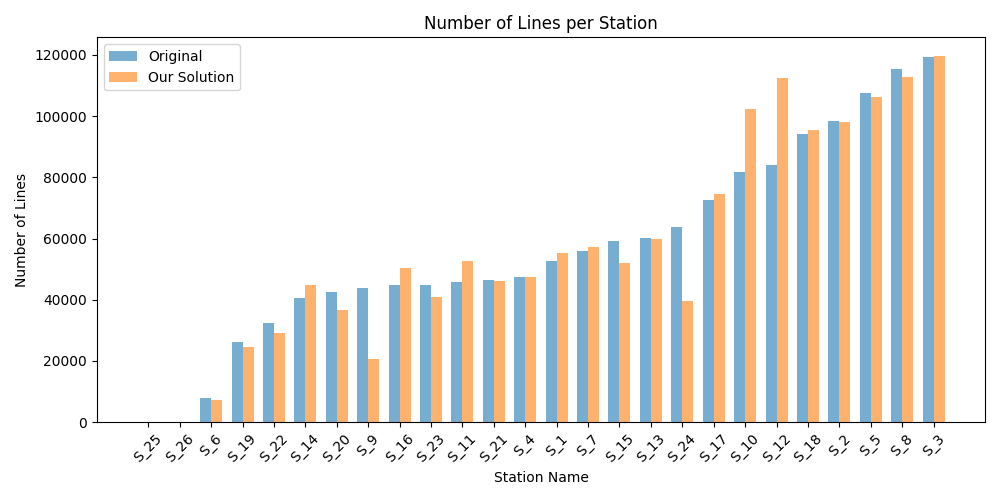
\includegraphics[width=0.49\linewidth]{Images_CSLAP/r4_number_of_lines_per_station.png}\hfill
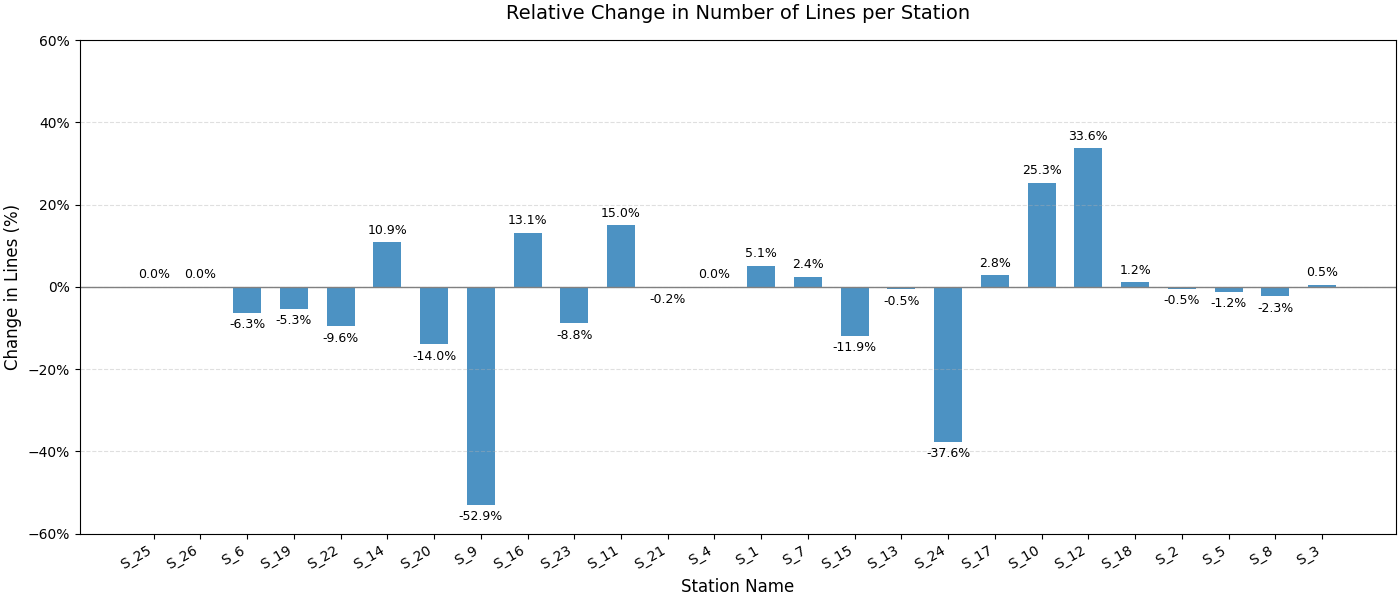
\includegraphics[width=0.49\linewidth]{Images_CSLAP/r5_pct_change_lines_per_station.png}
\caption{Lines per station (left) and relative change in utilisation (right) for the heuristic layout against the original. Several stations move well past their capacity.}
\label{fig:wl_heur}
\end{figure}

\begin{figure}[t]
\centering
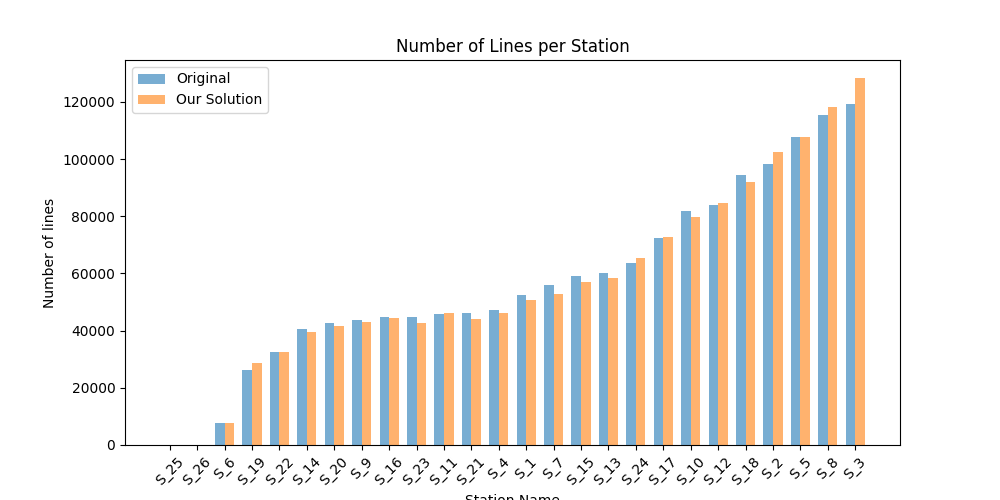
\includegraphics[width=0.49\linewidth]{Images_CSLAP/Hexaly_number_of_lines_per_station.png}\hfill
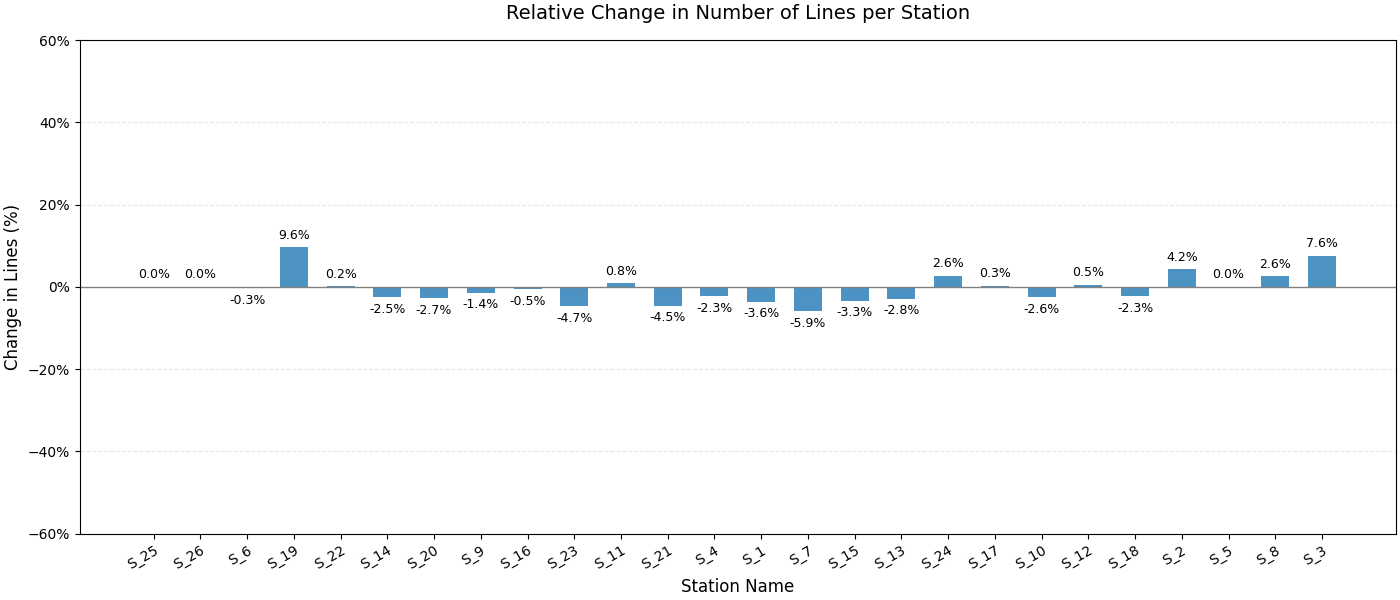
\includegraphics[width=0.49\linewidth]{Images_CSLAP/Hexaly_pt_relative_change_number_of_lines_per_station.png}
\caption{Lines per station (left) and relative change in utilisation (right) for the set-variable layout against the original. The relative change stays inside the operational slack on every station.}
\label{fig:wl_milp}
\end{figure}

\subsection{Robustness on unseen weeks}
A layout is optimised once and then operated as demand evolves, so we test out of sample. The dataset spans 13 weeks. In the first test the model sees only the first 10 weeks and is evaluated on the last 3; in the second it sees the first 8 and is evaluated on the last 5. Each layout is compared with the original placement and with an oracle layout optimised directly on the test weeks with perfect knowledge (Table~\ref{tab:temporal}). This out-of-sample design follows robustness practice in storage assignment, where an implementable policy is contrasted with a perfect-information oracle \citep{lee2020cie, wang2020}. Using 10 weeks of history cuts visits by 6.6 per cent on the held-out weeks, against 12.1 per cent for the oracle; using 8 weeks cuts visits by 7.4 per cent, against 10.2 per cent. The recent past therefore captures most, though not all, of the structural affinity benefit, which is enough for a meaningful and durable gain on this site.

\begin{table}[t]
\centering
\tbl{Out-of-sample station-visit performance on held-out weeks.}
{\begin{tabular}{@{}llrr@{}}
\toprule
Test period & Layout (training period) & Total visits & Mean visits \\
\midrule
\multirow{3}{*}{Last 3 weeks}
 & Original placement & 265{,}876 & 4.052 \\
 & Optimised on first 10 weeks & 248{,}358 & 3.785 \\
 & Oracle (optimised on last 3 weeks) & 233{,}728 & 3.562 \\
\midrule
\multirow{3}{*}{Last 5 weeks}
 & Original placement & 423{,}593 & 3.926 \\
 & Optimised on first 8 weeks & 392{,}318 & 3.636 \\
 & Oracle (optimised on last 5 weeks) & 380{,}356 & 3.525 \\
\bottomrule
\end{tabular}}
\label{tab:temporal}
\end{table}

\subsection{Bounded reassignment}\label{sec:reassign}
An established facility cannot absorb a disruptive re-slotting wave \citep{chabot2024reassignment}, so we bound how many products may move. Let $s'(p)$ be the legacy station of product $p$. Adding the single constraint
\begin{equation}
\sum_{p \in P} x_{p,\,s'(p)} \ \ge\ |P| - k
\label{eq:reassign}
\end{equation}
limits the number of relocated products to at most $k$. We solve the industrial instance for $k \in \{250, 500, 1000, 2000, 5000\}$ under a one-hour budget each and contrast the result with the legacy layout ($k=0$) and with the full re-optimisation that reached 917,465 visits under a 10-hour budget (Table~\ref{tab:reassign}, Figure~\ref{fig:ksweep}).

\begin{table}[t]
\centering
\tbl{Bounded-reassignment trade-off on the industrial instance. ``\% of full benefit'' is the reduction relative to the 145,042-visit full re-optimisation; the last column counts stations exceeding their cap.}
{\small\begin{tabular}{@{}lrrrrr@{}}
\toprule
Relocation cap & \% catalogue & Total visits & Reduction & \% of full benefit & WL-viol.\ stations \\
\midrule
Legacy ($k=0$) & 0\% & 1{,}062{,}507 & -- & -- & 0 \\
$k=250$        & 1.1\% & 1{,}061{,}302 & 1{,}205 & 0.8\% & 0 \\
$k=500$        & 2.3\% & 1{,}060{,}120 & 2{,}387 & 1.6\% & 0 \\
$k=1{,}000$    & 4.6\% & 1{,}056{,}412 & 6{,}095 & 4.2\% & 0 \\
$k=2{,}000$    & 9.1\% & 1{,}049{,}730 & 12{,}777 & 8.8\% & 0 \\
$k=5{,}000$    & 22.9\% & 1{,}034{,}735 & 27{,}772 & 19.2\% & 0 \\
Full re-opt.   & --     & 917{,}465 & 145{,}042 & 100\% & 0 \\
\bottomrule
\end{tabular}}
\label{tab:reassign}
\end{table}

\begin{figure}[t]
\centering
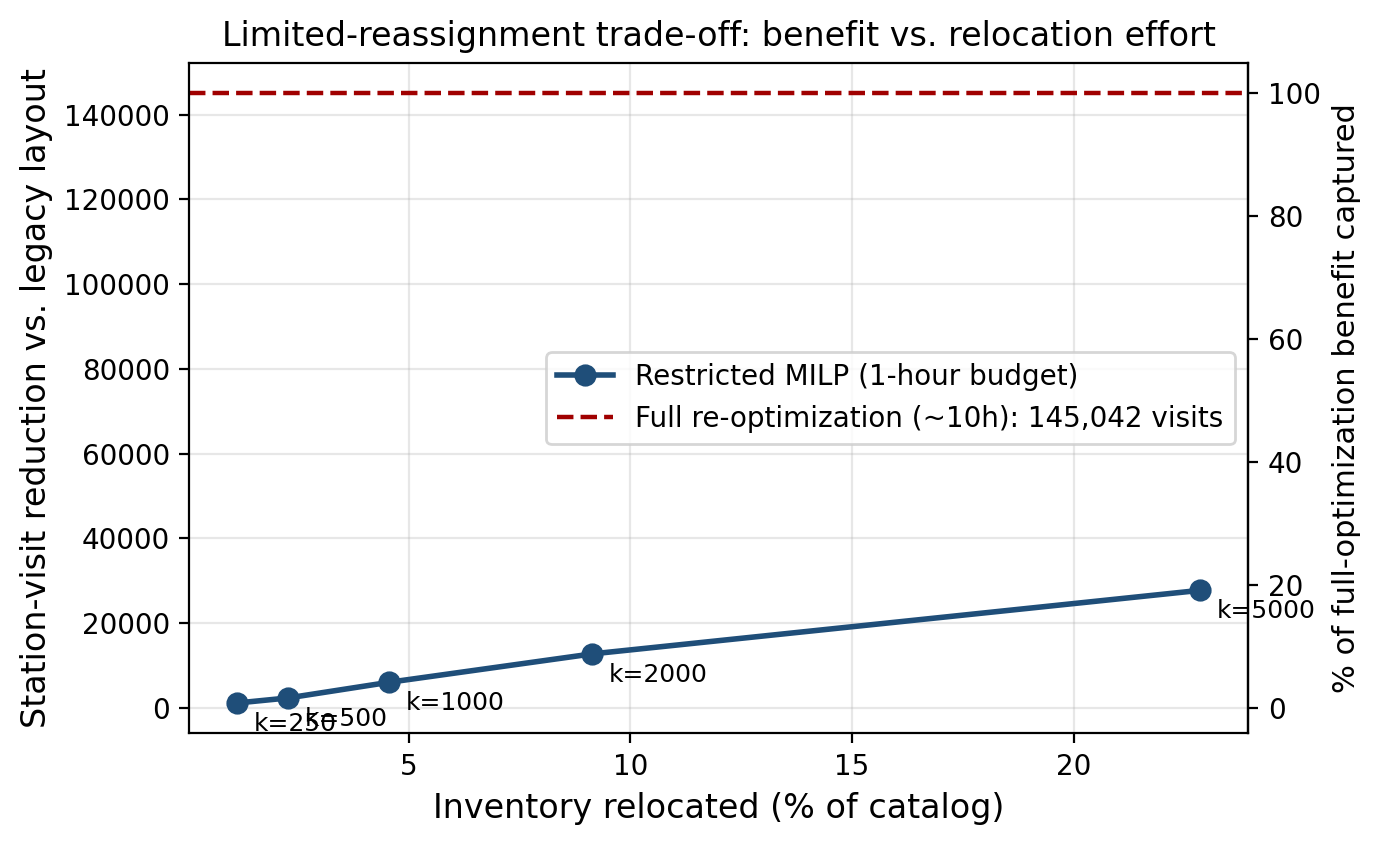
\includegraphics[width=0.7\linewidth]{Images_CSLAP/reassignment_ksweep_curve.png}
\caption{Station-visit reduction against the share of the catalogue relocated. The dashed line marks the full re-optimisation benefit. The benefit accrues gradually with relocation effort rather than concentrating in a small fraction of moves.}
\label{fig:ksweep}
\end{figure}

Two findings emerge. The benefit of bounded re-slotting accrues roughly in step with the relocation effort: relocating 2.3 per cent of the catalogue captures 1.6 per cent of the full reduction, and relocating 22.9 per cent captures 19.2 per cent. No small subset of moves captures a disproportionate share, so most of the gain in the full solution still comes from a large rearrangement that a tight budget cannot reproduce. The curve quantifies what a manager gives up by limiting disruption, and lets the budget $k$ be matched to available labour against a known marginal benefit. Every bounded layout also stays feasible: at each cap the solver keeps all 26 stations within both capacity and workload, and it leaves the site's engineered balance almost intact, with the busiest station load and the spread of utilisation barely moving from their legacy values. The whole curve can therefore be deployed as it stands, without a separate workload filter or a longer overnight solve, because each station's residual time budget is reserved for the frozen low-frequency products before the bounded search runs.

% =====================================================================
\section{Managerial insights for decision makers in industry}\label{sec:managerial}
% =====================================================================
The results carry four messages for warehouse operations.

Track station visits as a slotting indicator. In conveyor and zone-routing systems each diversion generates mechanical queueing and handling delay, so stops per order expose congestion that a distance metric hides. On Company~A the original layout required 1,062,507 visits over a 66-day quarter, about 16,099 stops per day. The set-variable layout cuts this to 917,465, a 13.7 per cent structural reduction, or about 2,198 fewer stops per day.

Read the labour effect as a planning figure, not a measured one. Multiplying the 145,042 eliminated visits by a fixed mechanical time per visit frees about nine working days of picker and conveyor dwell per quarter. This is a linear projection under a fixed time per visit; it does not yet model queueing, and a discrete-event study is needed to confirm it (Section~\ref{sec:perspectives}). Stated as a planning figure it still gives operations a concrete target.

Match the tool to the decision. For a scheduled, quarterly re-slotting, the set-variable approach produces the highest-quality layout we obtain while holding every station within capacity. For a fast, exploratory pass where balance can be checked afterwards, the clustering heuristic runs in seconds, with the understanding that its raw output must be filtered for workload before use.

Improve continuously without a shutdown. The bounded-reassignment model lets a site move only as many products as its workforce can handle in one cycle. Table~\ref{tab:reassign} gives the manager the trade-off curve directly, so the relocation budget can be set against the marginal benefit rather than guessed. Every point on that curve holds all stations within capacity and workload, so the chosen budget can be deployed as it is, and the rolling re-optimisation on an 8 to 10-week window keeps the layout current with limited engineering effort.

% =====================================================================
\section{Research perspectives}\label{sec:perspectives}
% =====================================================================
Three tracks extend this work. The first is the pricing subproblem of the column-generation framework, which is the factor that limits its scale. Stabilisation of the duals, machine-learning-guided pricing, and metaheuristic post-processing of fractional columns are candidate routes to bring its bounds to facility scale. The second is product geometry. The model counts a product as one unit of a station's capacity; replacing that count with a per-product footprint $a_p$ in constraint \eqref{eq:cap}, and coupling it to the temporal budget \eqref{eq:wl}, would let three-dimensional packing limits enter without changing the structure of the programme. The third is the visit-to-throughput link. We balance workload, which lowers expected queueing, but we do not yet model the queue. Feeding the optimised layout into a high-fidelity discrete-event simulation would quantify micro-level queue states and convert the planning figures of Section~\ref{sec:managerial} into measured throughput, and would also open the door to stochastic demand and real-time routing.

% =====================================================================
\section{Conclusion}\label{sec:conclusion}
% =====================================================================
We posed the correlated storage location assignment problem for automated pick-and-pass warehouses with station visits as the objective and hard capacity and workload limits. The objective is piecewise constant, which stalls branch-and-bound and metaheuristic search at scale. Pairing a set-variable reformulation with a hybrid local-search engine clears that barrier: it is the best feasible method across synthetic instances of 50 to 2000 products, with a margin over the literature baselines that widens with size, and it lowers station visits on a real 21,877-product warehouse by 13.7 per cent while keeping every station within capacity. A bounded-reassignment extension maps the trade-off between re-slotting effort and throughput, which makes the gains deployable on an active site without a shutdown.

% ---------------------------------------------------------------------
% BACK MATTER (IJPR order)
% ---------------------------------------------------------------------
\section*{Acknowledgements}
This research was carried out with the support of the Association Nationale de la Recherche et de la Technologie (ANRT), Savoye, and the Universit\'{e} de technologie de Compi\`{e}gne. The authors thank the operational teams at Company~A for the dataset and for their insight into the picking process.

\section*{Author contributions}
The authors confirm contribution to the paper as follows. Ermal Belul, Marwane Bouznif, Dritan Nace, and Antoine Jouglet were involved in the conception, design, and modelling of the framework; Ermal Belul developed the software and analysed the empirical data; Ermal Belul drafted the manuscript, and Marwane Bouznif, Dritan Nace, and Antoine Jouglet critically revised it for intellectual content. All authors gave final approval of the version to be published and agree to be accountable for all aspects of the work.

\section*{Disclosure statement}
The authors report there are no competing interests to declare.

\section*{Declaration of generative AI use}
During the preparation of this work the authors used a generative AI assistant in order to refine language and improve readability. After using this tool the authors reviewed and edited the content as needed and take full responsibility for the content of the published article.

\section*{Notes on contributors}
\textit{Ermal Belul} is a doctoral researcher at the Universit\'{e} de technologie de Compi\`{e}gne (Heudiasyc laboratory) and Savoye, working on decision-support tools under uncertainty for intralogistics, with a focus on storage assignment and warehouse optimisation.

\textit{Marwane Bouznif} is a research and development engineer at Savoye, working on optimisation methods for automated warehouse systems.

\textit{Dritan Nace} is a professor at the Universit\'{e} de technologie de Compi\`{e}gne (Heudiasyc laboratory). His research covers combinatorial optimisation, network design, and robust optimisation.

\textit{Antoine Jouglet} is a professor at the Universit\'{e} de technologie de Compi\`{e}gne (Heudiasyc laboratory). His research covers scheduling, constraint programming, and combinatorial optimisation.

\section*{Data availability statement}
This journal applies the Taylor \& Francis ``share upon reasonable request'' data sharing policy. The synthetic datasets and the algorithm source code are openly available at the repository linked from the submission; the de-anonymised permanent link will be provided on acceptance. The real-world industrial dataset from Company~A cannot be made public due to commercial confidentiality restrictions and may be requested from the authors under reasonable operational conditions.

% ---------------------------------------------------------------------
% References (APA via apacite)
% ---------------------------------------------------------------------
\bibliographystyle{apacite}
\bibliography{IJPR_CSLAP}

% ---------------------------------------------------------------------
% APPENDIX
% ---------------------------------------------------------------------
\appendix
\section{Greedy clustering heuristic}\label{app:heuristic}
\begin{algorithm}[t]
\caption{Greedy product clustering and station assignment}
\label{alg:heuristic}
\begin{algorithmic}[1]
\State \textbf{Input:} products $P$, orders $O$, stations $S$; thresholds derived from $N=|P|$.
\State \textbf{Step 1 (preprocessing).} Keep products above the frequency floor. For each multi-item order, form product pairs; keep pairs whose co-occurrence count clears the minimum and whose conditional share clears the kept-edge ratio. Sort kept pairs by decreasing co-occurrence.
\State \textbf{Step 2 (community formation).} Initialise the community set empty. While candidate pairs remain, take the top pair as a new community, then repeatedly add the product with the highest aggregate co-occurrence with the community until the size bound is reached; remove from the candidate list every pair containing an added product.
\State \textbf{Step 3 (post-processing).} Place each low-frequency product into the community with which it most co-occurs and which has room. Group any remaining products into a new community within the size bound.
\State \textbf{Step 4 (station assignment).} Rank communities by cumulative demand. For each community, sort stations by historical preference and assign it to the first preferred station with capacity $\zeta_s$ to hold it; if none can hold it whole, split it across stations so as to keep the most correlated products together.
\State \textbf{Output:} a product-to-station assignment.
\end{algorithmic}
\end{algorithm}

\end{document}
